
\begin{frame}[fragile]{Lectura de Códigos QR en Android}
\textbf{¿Qué es un decodificador QR?}

\begin{itemize}
    \item Permite leer y decodificar información contenida en códigos QR usando la cámara del dispositivo.
    \item Se utiliza en aplicaciones de pagos, accesos, inventarios, entre otros.
\end{itemize}

\textbf{Uso de librerías externas:}
\begin{itemize}
    \item Android no incluye un lector QR nativo completo.
    \item Se pueden integrar librerías como \textbf{ZXing} o \textbf{ML Kit}.

\scriptsize
\begin{minted}{groovy}
dependencies {
    implementation 'com.journeyapps:zxing-android-embedded:4.3.0'
    implementation 'com.google.zxing:core:3.5.1'
}
\end{minted}

\end{itemize}

\textbf{Ventajas:}
\begin{itemize}
    \item Integración rápida y sencilla.
    \item Soporte para múltiples formatos de códigos.
\end{itemize}

\end{frame}



\begin{frame}[fragile]
\frametitle{Demo 13: Decodificacion de Codigos QR con Camara }
\begin{columns}
\column{0.80\linewidth}
Del Repositorio Github:
\begin{itemize}
\item Copiar el archivo \textit{MainActivity\_Demo13.java} (dentro del Folder códigosJAVA) al mismo directorio donde esta el MainActivity.java
\item Copiar el archivo \textit{activity\_main\_demo13.xml} (dentro del Folder Carpeta\_layout) al mismo directorio donde esta el activity\_main.xml
%\item Copiar el archivo \textit{custom\_dialog.xml} (dentro del Folder Carpeta\_layout) al mismo directorio donde esta el activity\_main.xml.
\item Modificar en el archivo \textit{AndroidManifest.xml} la cadena \textit{.MainActivity\_Demo12} por \textit{.MainActivity\_Demo13}.
\item Agregar la siguiente linea: \textit{implementation (``com.journeyapps:zxing-android-embedded:4.3.0'')}, al final de la seccion Dependencies del archivo Build.graddle.kts (Module: App).

%\item Ir a la linea 22 de archivo del archivo \textit{MainActivity\_Demo09.java}, poner el cursos en la palabra (en Rojo) \textit{documentfile}, presionar la combinación ALT+ENTER, y seleccionar de la lista desplegable la opcion ``Add dependency on ....''. Esto quitará el error y hara los ajustes necesarios. 
\end{itemize}

%\begin{block}{Demo \#09}
%Un App que permite escribir el contenido de un EditText a un archivo y cargar el contenido de cualquier archivo en el EditText
%\end{block}


\column{0.20\linewidth}

\begin{center}
 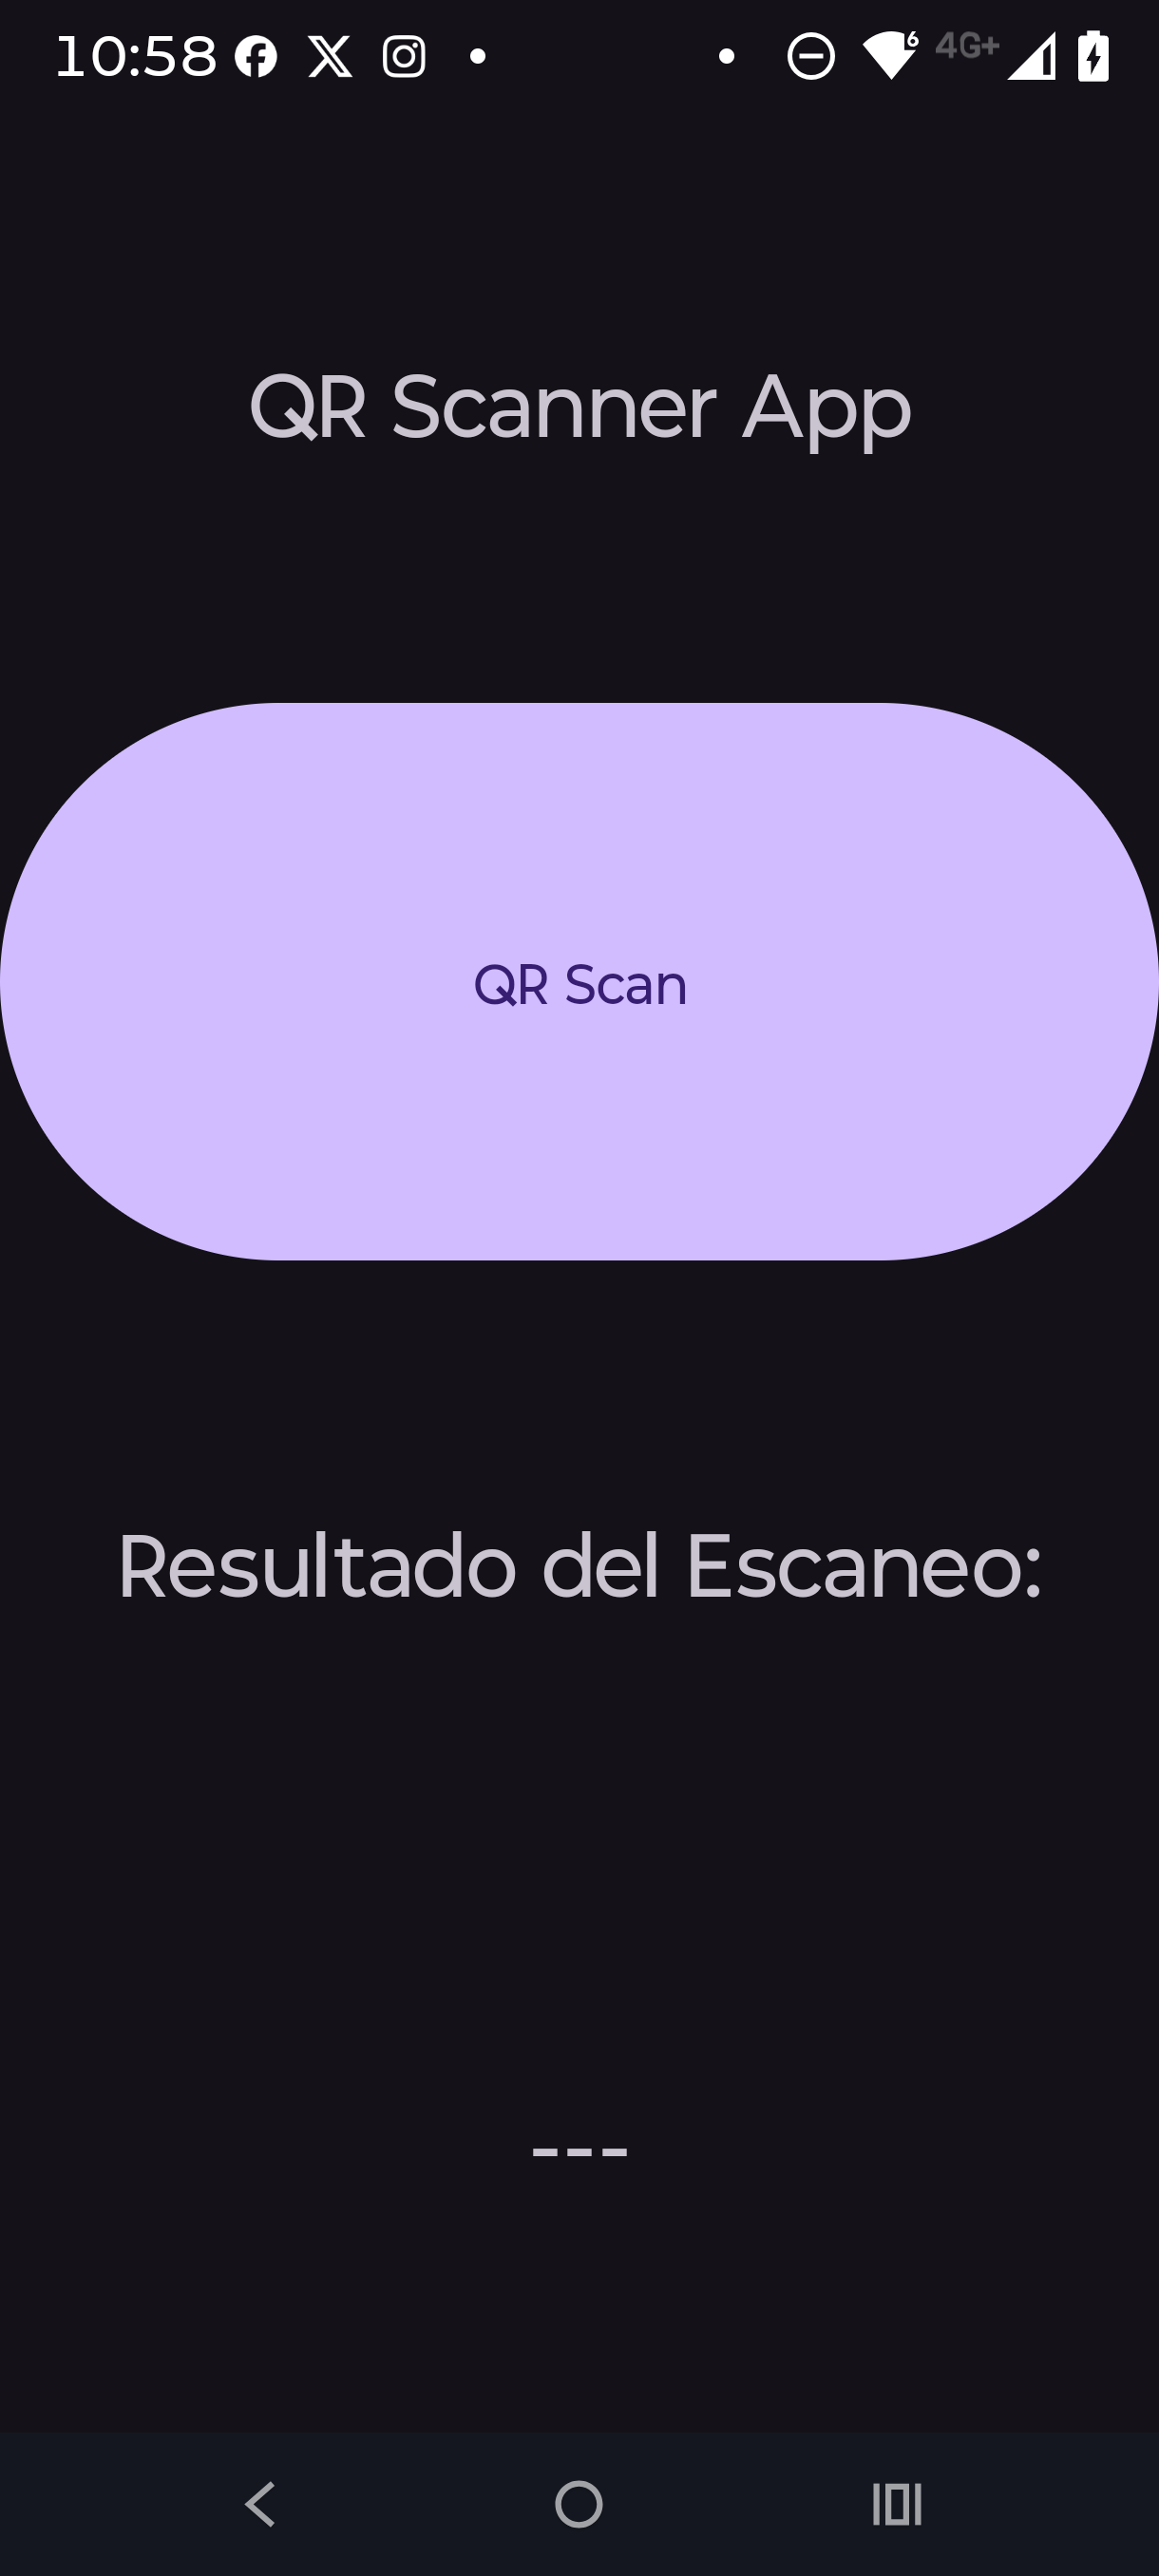
\includegraphics[width=0.98\textwidth]{02_TallerCBTis/figs/Demo13}
\end{center}

\end{columns}

\end{frame}

